\documentclass[pdflatex,compress,mathserif]{beamer}

%\usetheme[dark,framenumber,totalframenumber]{ElektroITK}
\usetheme[darktitle,framenumber,totalframenumber]{ElektroITK}

\usepackage[utf8]{inputenc}
\usepackage[T1]{fontenc}
\usepackage{lmodern}
\usepackage[bahasai]{babel}
\usepackage{amsmath}
\usepackage{amsfonts}
\usepackage{amssymb}
\usepackage{graphicx}
\usepackage{multicol}
\usepackage{lipsum}

\newcommand*{\Scale}[2][4]{\scalebox{#1}{$#2$}}%

\title{PEMODELAN JARINGAN KOMUNIKASI}
\subtitle{The Life of a Packet}

\author{Tim Dosen Pengampu}

\begin{document}

\maketitle

\section{DNS - The Domain Name System}

\begin{frame}
	\frametitle{OSI Reference Model - Encapsulation}
	\begin{center}
		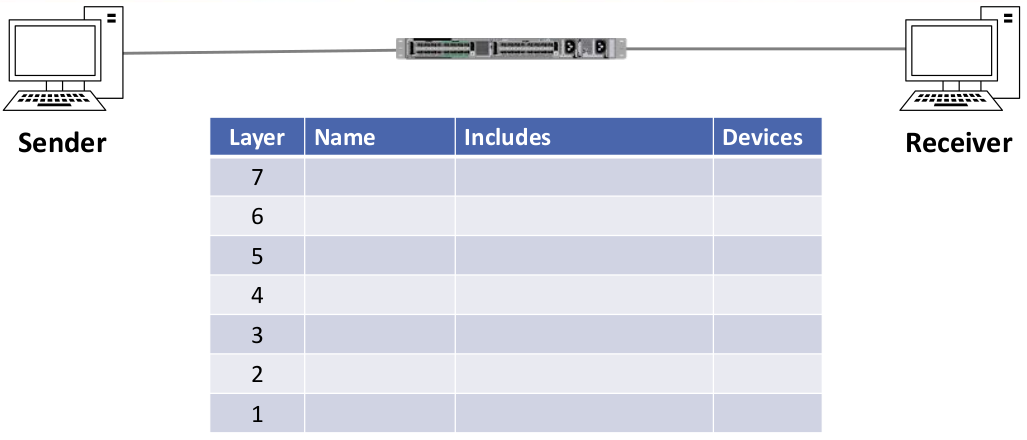
\includegraphics[width=\linewidth]{img/img01}
	\end{center}
\end{frame}

\begin{frame}{OSI Reference Model - Encapsulation}
	\begin{center}
		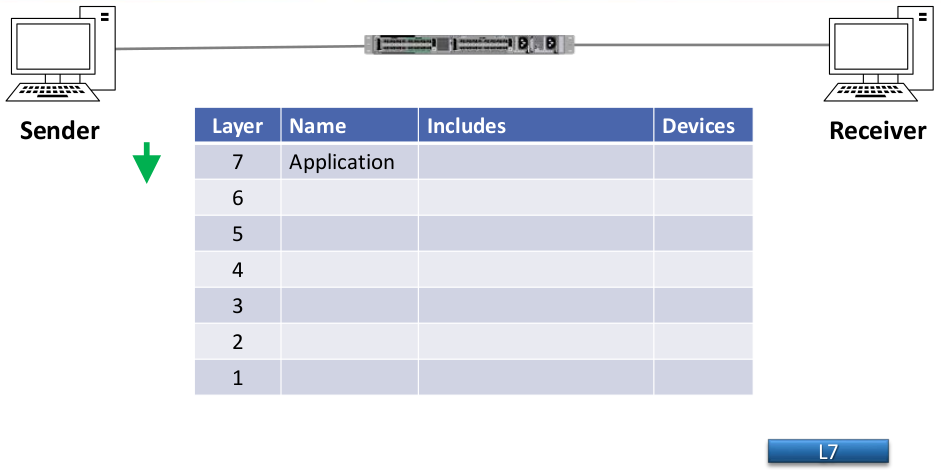
\includegraphics[width=\linewidth]{img/img02}
	\end{center}
\end{frame}

\begin{frame}{OSI Reference Model - Encapsulation}
	\begin{center}
		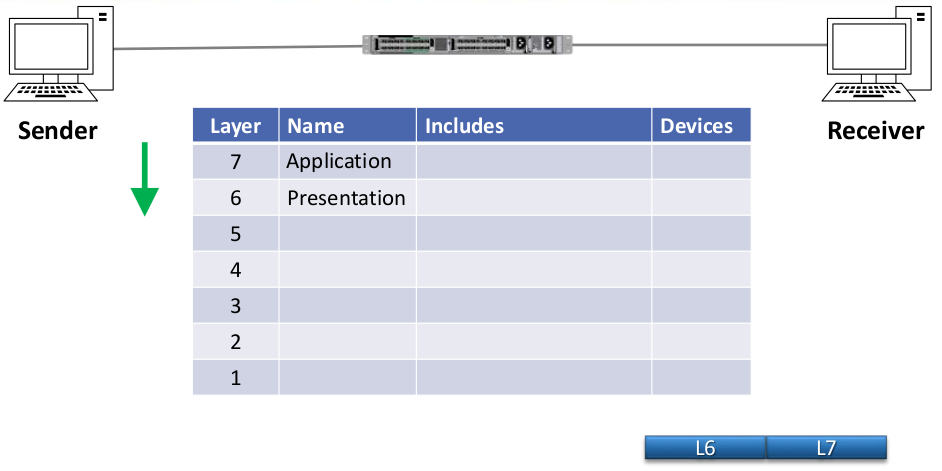
\includegraphics[width=\linewidth]{img/img03}
	\end{center}
\end{frame}

\begin{frame}{OSI Reference Model - Encapsulation}
	\begin{center}
		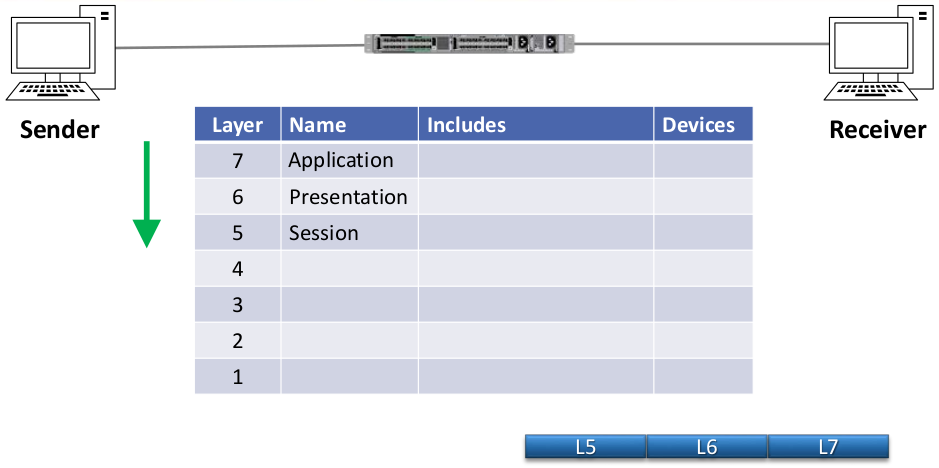
\includegraphics[width=\linewidth]{img/img04}
	\end{center}
\end{frame}

\begin{frame}{OSI Reference Model - Encapsulation}
	\begin{center}
		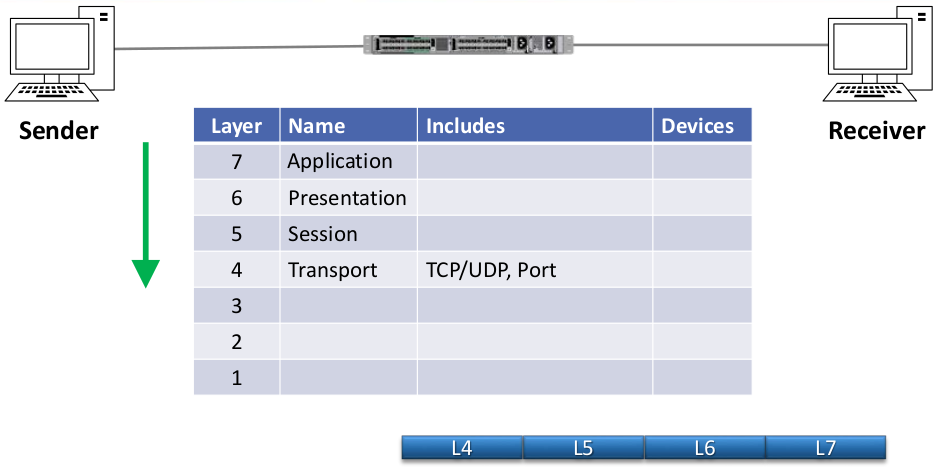
\includegraphics[width=\linewidth]{img/img05}
	\end{center}
\end{frame}

\begin{frame}{OSI Reference Model - Encapsulation}
	\begin{center}
		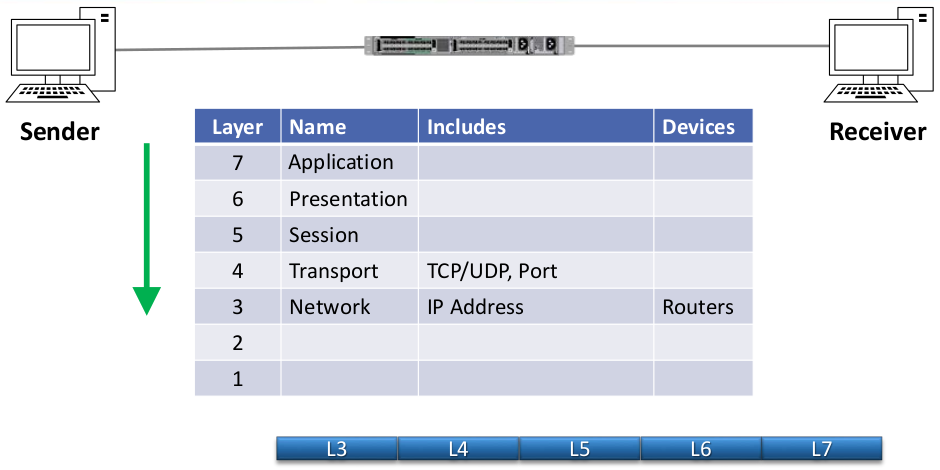
\includegraphics[width=\linewidth]{img/img06}
	\end{center}
\end{frame}

\begin{frame}
	\frametitle{The Domain Name System}
	\begin{itemize}
		\item The Domain Name System (DNS) resolves a Fully Qualified Domain Name (FQDN) such as www.cisco.com to an IP address.
		\item Enterprises will typically have an internal DNS server which can resolve the IP addresses of internal hosts.
		\item Hosts will send their DNS queries to this server.
		\item If the internal DNS server cannot resolve a query, it will forward the request out to public DNS servers on the Internet.
		\item DNS requests are sent using UDP port 53 (and can fail over to TCP).
	\end{itemize}
\end{frame}

\section{DNS on Cisco Routers}

\begin{frame}
	\frametitle{Router DNS Commands}
	\begin{itemize}
		\item DNS Client:
		\item[] \texttt{ip domain-lookup}
		\item[] \texttt{ip name-server 172.23.4.1}
		\item[] \texttt{ip domain-name flackboxA.lab} (primary domain name)
		\item[] \texttt{ip domain-list flackboxB.lab} (additional DNS suffixes to search)
		\item Additional DNS Server Commands:
		\item[] \texttt{ip dns server}
		\item[] \texttt{ip host LinuxA 172.23.4.2}
	\end{itemize}
\end{frame}

\section{ARP - Address Resolution Protocol}

\begin{frame}
	\frametitle{OSI Reference Model - Encapsulation}
	\begin{center}
		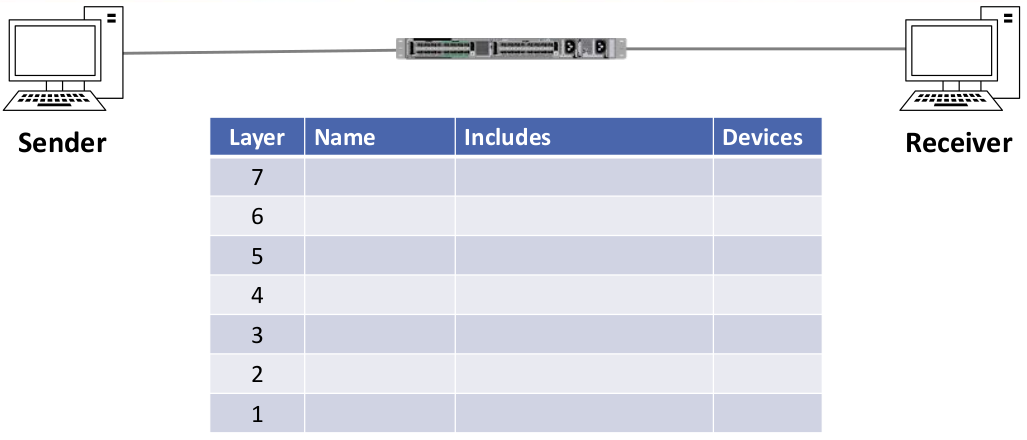
\includegraphics[width=\linewidth]{img/img01}
	\end{center}
\end{frame}

\begin{frame}{OSI Reference Model - Encapsulation}
	\begin{center}
		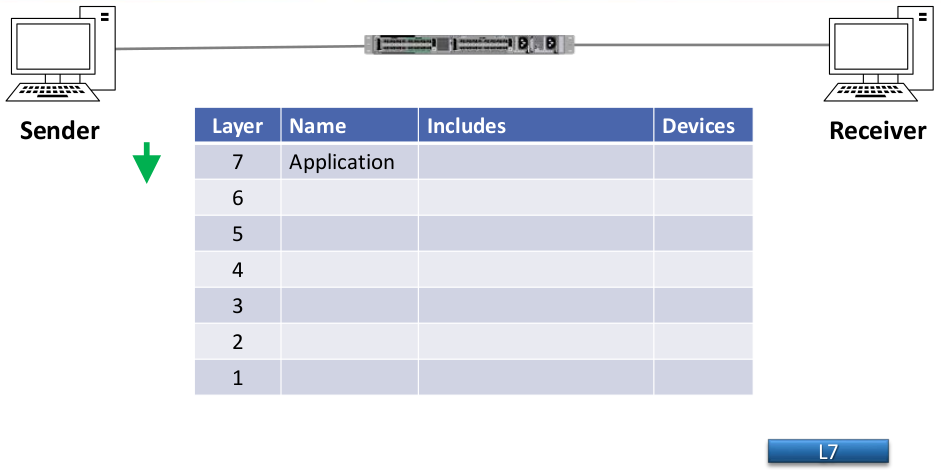
\includegraphics[width=\linewidth]{img/img02}
	\end{center}
\end{frame}

\begin{frame}{OSI Reference Model - Encapsulation}
	\begin{center}
		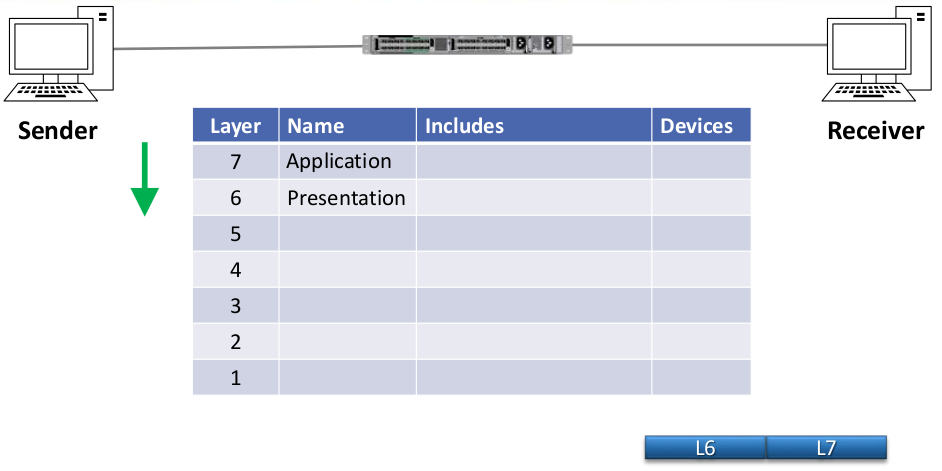
\includegraphics[width=\linewidth]{img/img03}
	\end{center}
\end{frame}

\begin{frame}{OSI Reference Model - Encapsulation}
	\begin{center}
		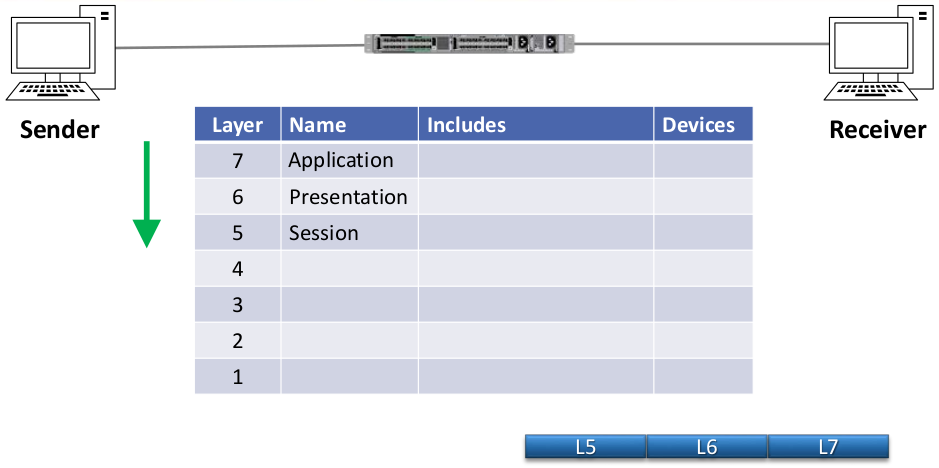
\includegraphics[width=\linewidth]{img/img04}
	\end{center}
\end{frame}

\begin{frame}{OSI Reference Model - Encapsulation}
	\begin{center}
		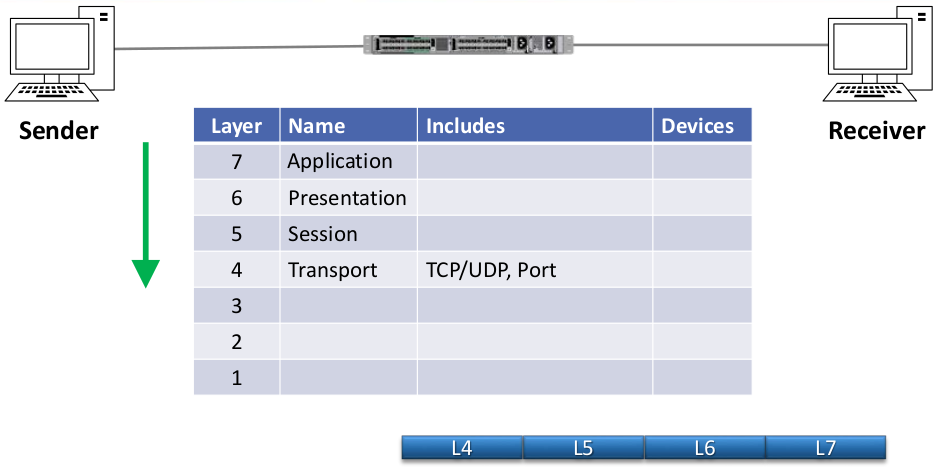
\includegraphics[width=\linewidth]{img/img05}
	\end{center}
\end{frame}

\begin{frame}{OSI Reference Model - Encapsulation}
	\begin{center}
		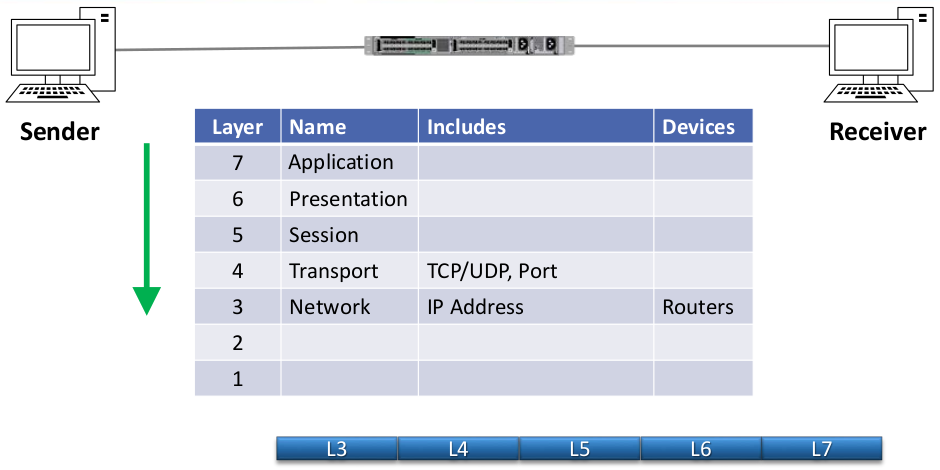
\includegraphics[width=\linewidth]{img/img06}
	\end{center}
\end{frame}

\begin{frame}{OSI Reference Model - Encapsulation}
	\begin{center}
		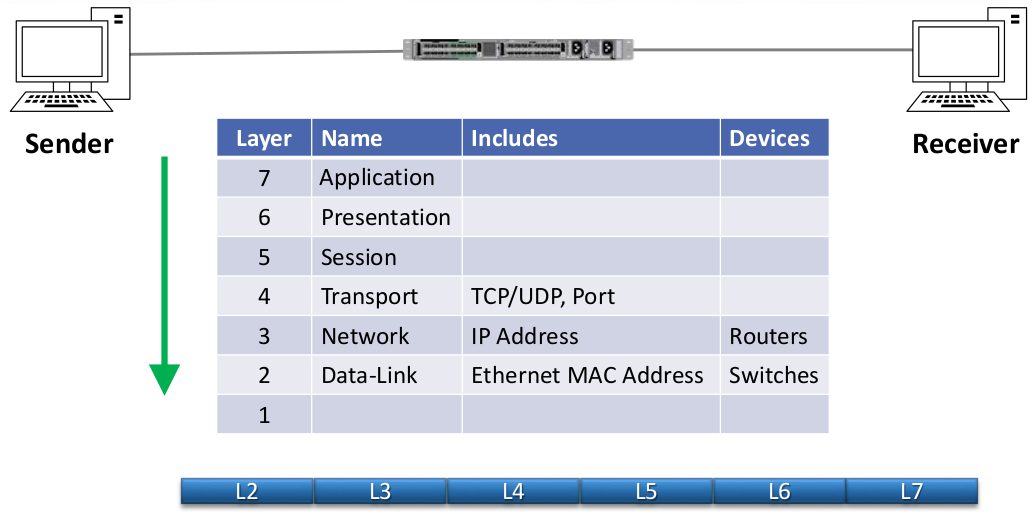
\includegraphics[width=\linewidth]{img/img07}
	\end{center}
\end{frame}



\end{document}
